\documentclass[10pt]{article}

%%%%%%%%%%%%%%%%%%%%%%%%%%%%%%%%%%%%%%%%%%%%%%%%%%%%%%%%%%%%%%%%%%%%%%
% IISE Annual Conference Proceedings Template
% Based on official IISE Annual Conference formatting guidelines
%%%%%%%%%%%%%%%%%%%%%%%%%%%%%%%%%%%%%%%%%%%%%%%%%%%%%%%%%%%%%%%%%%%%%%

%%%%% Page Setup %%%%%%%%%%%%%%%%%%%%%%%%%%%%%%%%%%%%%%%%%%%%%%%%%%%%%
\usepackage[letterpaper, margin=1in, headheight=25pt]{geometry}
\usepackage{times}           % Times New Roman font
\usepackage{graphicx}        % For figures
\usepackage{amsmath}         % For equations
\usepackage{cite}            % For IEEE style citations
\usepackage{url}             % For URLs in references
\usepackage{hyperref}        % For clickable links
\usepackage{fancyhdr}        % For headers
\usepackage{titlesec}        % For section formatting
\usepackage{caption}         % For caption formatting
\usepackage{parskip}         % For paragraph spacing
\usepackage{enumitem}        % For bullet formatting
\usepackage{etoolbox}        % For patching environments
\usepackage{microtype}       % Microtypography
\usepackage{booktabs}        % Professional tables
\usepackage{amssymb}         % For \checkmark in tables

%%%%% Hyperref Settings %%%%%%%%%%%%%%%%%%%%%%%%%%%%%%%%%%%%%%%%%%%%%%
\hypersetup{
    colorlinks=true,
    linkcolor=black,
    urlcolor=blue,
    citecolor=black,
    pdfborder={0 0 0}
}

%%%%% Paragraph and Spacing Settings %%%%%%%%%%%%%%%%%%%%%%%%%%%%%%%%%
\setlength{\parindent}{0pt}
\setlength{\parskip}{10pt}
\linespread{1.0}
\pagestyle{fancy}
\fancyhf{}
\renewcommand{\headrulewidth}{0pt}
\renewcommand{\footrulewidth}{0pt}

%%%%% First Page Header %%%%%%%%%%%%%%%%%%%%%%%%%%%%%%%%%%%%%%%%%%%%%%
\fancypagestyle{firstpage}{%
    \fancyhf{}
    \fancyhead[L]{{\fontsize{10}{12}\selectfont 
    Proceedings of the 2026 IISE Annual Conference \\
    H. Xiao, H.E. Romeijn, Z. Shen, M. Zhou, eds.}}
    \renewcommand{\headrulewidth}{0pt}
}

%%%%% Section Formatting %%%%%%%%%%%%%%%%%%%%%%%%%%%%%%%%%%%%%%%%%%%%
\titleformat{\section}
    {\normalfont\fontsize{12}{14}\bfseries\selectfont}
    {\thesection.}{0.5em}{}
\titlespacing*{\section}{0pt}{10pt}{0pt}

\titleformat{\subsection}
    {\normalfont\fontsize{10}{12}\bfseries\selectfont}
    {\thesubsection}{0.5em}{}
\titlespacing*{\subsection}{0pt}{10pt}{0pt}

\titleformat{\subsubsection}
    {\normalfont\fontsize{10}{12}\bfseries\selectfont}
    {\thesubsubsection}{0.5em}{}
\titlespacing*{\subsubsection}{0pt}{10pt}{0pt}

%%%%% Caption Formatting %%%%%%%%%%%%%%%%%%%%%%%%%%%%%%%%%%%%%%%%%%%%%
\captionsetup[table]{
    position=top, justification=centering,
    singlelinecheck=true, labelsep=colon,
    font={normalsize}, skip=10pt
}
\captionsetup[figure]{
    position=bottom, justification=centering,
    singlelinecheck=true, labelsep=colon,
    font={normalsize}, skip=10pt
}
\setlength{\textfloatsep}{12pt plus 2pt minus 4pt}
\setlength{\floatsep}{12pt plus 2pt minus 4pt}

%%%%% Bullet List Formatting %%%%%%%%%%%%%%%%%%%%%%%%%%%%%%%%%%%%%%%%%
\setlist[itemize,1]{label=\textbullet, leftmargin=0.5in}
\setlist[itemize,2]{label=$\circ$, leftmargin=0.75in}

%%%%% Blind Review Flag %%%%%%%%%%%%%%%%%%%%%%%%%%%%%%%%%%%%%%%%%%%%%%
\def\blind{1}
\def\final{0}
\if1\final
    \fancyhead[C]{\textit{Author Last Names}}
\fi

\begin{document}
\microtypesetup{nopatch=item}
\thispagestyle{firstpage}

%%%%% TITLE %%%%%%%%%%%%%%%%%%%%%%%%%%%%%%%%%%%%%%%%%%%%%%%%%%%%%%%%%%
\if1\blind
\begin{center}
{\fontsize{16}{19}\bfseries\selectfont
A Modular Open-Source Digital Model Architecture for Bioprocess Design: Validation through Stochastic Simulation of an Isolated Soy Protein Plant}

\vspace{10pt}

\if0\final
{\fontsize{12}{14}\bfseries\selectfont Abstract ID: 1234}
\vspace{10pt}
\fi

{\fontsize{10}{12}\selectfont Author information is purposely removed for blind review}
\end{center}
\fi

\if0\blind
\begin{center}
{\fontsize{16}{19}\bfseries\selectfont
A Modular Open-Source Digital Model Architecture for Bioprocess Design: Validation through Stochastic Simulation of an Isolated Soy Protein Plant}

\vspace{10pt}

\if0\final
{\fontsize{12}{14}\bfseries\selectfont Abstract ID: 1234}
\vspace{10pt}
\fi

{\fontsize{10}{12}\selectfont
Samuel Aguilera$^{a}$ \\
\vspace{5pt}
$^{a}$Department of Industrial Engineering, Universidad Cat\'olica Boliviana ``San Pablo'', Bolivia \\
\texttt{samuel.aguilera@ucb.edu.bo}}
\end{center}
\fi

\vspace{10pt}
\microtypesetup{patch=item}

%%%%% ABSTRACT %%%%%%%%%%%%%%%%%%%%%%%%%%%%%%%%%%%%%%%%%%%%%%%%%%%%%%%
\begin{center}
{\fontsize{12}{14}\bfseries\selectfont Abstract}
\end{center}

There is growing interest in digital twins for bioprocesses. However, most frameworks work at the shadow or twin level and need IoT infrastructure, which is not available during early design. This paper presents a modular, open-source digital model architecture at Kritzinger's ``Digital Model'' level. The system has four decoupled Python modules: a phenomenological kernel with mass and energy balances for each unit operation, a constraint engine that checks equipment capacity limits, a configuration layer with automatic range validation, and a real-time visualization dashboard. The architecture is validated through an Isolated Soy Protein (ISP) plant case study at 1,000 kg/h. A Monte Carlo campaign of 100,000 runs on the initial design gave only 4.70\% success. Based on a bottleneck analysis, equipment was resized. A second campaign of 300,000 runs achieved 99.88\% success (3.03$\sigma$), with 19.5\% energy savings from reverse osmosis pre-concentration. All eleven unit tests pass, which confirms numerical integrity.

%%%%% KEYWORDS %%%%%%%%%%%%%%%%%%%%%%%%%%%%%%%%%%%%%%%%%%%%%%%%%%%%%%%
{\fontsize{12}{14}\bfseries\selectfont Keywords}\newline
{\fontsize{10}{12}\selectfont
Digital twin, open-source simulation, Monte Carlo, bioprocess design, Python}

%%%%%%%%%%%%%%%%%%%%%%%%%%%%%%%%%%%%%%%%%%%%%%%%%%%%%%%%%%%%%%%%%%%%%%
\section{Introduction}

Kritzinger et al.~\cite{kritzinger2018digital} define three levels of virtual integration: \textbf{Digital Model} (static, no automatic data exchange), \textbf{Digital Shadow} (one-way data flow from process to model), and \textbf{Digital Twin} (two-way data flow). Most reported work focuses on the upper two levels, but these depend on commercial data platforms that make independent replication difficult~\cite{gil2024survey}. There is a need for open-source platforms at the base level: the phenomenological Digital Model.

This work fills that need by presenting a modular, replicable Digital Model architecture in pure Python. It is at Kritzinger's first level: it does not need real-time data or IoT infrastructure. It can serve as a mathematically verifiable basis for future Digital Shadow or Twin development. The core uses conservation equations, not black-box models, which makes the model interpretable and adaptable to different processes~\cite{perry2019}.

The paper is organized as follows. Section~2 reviews related work. Section~3 describes the architecture. Section~4 covers replicability. Section~5 presents Monte Carlo validation on an ISP plant. Section~6 concludes and discusses future work.

\section{Related Work}

Several open-source digital twin frameworks have been developed. OpenTwins~\cite{robles2023opentwins} provides compositional DT development with Eclipse Ditto and Kubernetes. CoFMPy~\cite{friedrich2025cofmupy} enables FMI-based co-simulation with AI. DT-Forge~\cite{dtforge2025} offers a six-layer architecture for real-time telemetry. UniTwin~\cite{haussermann2024unitwin} provides containerized universal DTs. TumorTwin~\cite{tumortwin2025} targets personalized oncology with modular Python. In bioprocessing, Udugama et al.~\cite{udugama2023digital} propose multi-layer models for food processing, Gamero et al.~\cite{gamero2024data} introduce Lean Digital Twins for biorefineries, and Verboven et al.~\cite{verboven2020digital} lay the conceptual foundations for food processing DTs.

Table~\ref{tab:comparativa} compares these frameworks with our proposal. Most of them do not have statistical validation or automated unit testing. Our architecture is the only Digital Model that includes all four validation layers: phenomenological models, automated unit testing, stochastic analysis, and a real-world case study.

\begin{table}[!ht]
\centering
\caption{Comparison of digital twin frameworks.}
\label{tab:comparativa}
\small
\begin{tabular}{lccccccc}
\toprule
\textbf{Framework} & \textbf{Pure} & \textbf{Stat.} & \textbf{Unit} & \textbf{Phenom.} & \textbf{Integr.} & \textbf{UI} & \textbf{Real} \\
 & \textbf{Python} & \textbf{Valid.} & \textbf{Tests} & \textbf{Model} & \textbf{Level} & & \textbf{Case} \\
\midrule
This work & $\checkmark$ & $\checkmark$ & $\checkmark$ & $\checkmark$ & Model & $\checkmark$ & $\checkmark$ \\
OpenTwins & $\times$ & $\times$ & $\times$ & $\times$ & Twin & $\checkmark$ & $\checkmark$ \\
CoFMPy & $\checkmark$ & $\times$ & $\times$ & FMU ext. & Shadow & GUI & $\checkmark$ \\
DT-Forge & $\checkmark$ & $\times$ & $\times$ & Optional & Twin & $\times$ & $\times$ \\
UniTwin & $\times$ & $\times$ & $\times$ & $\times$ & Twin & $\checkmark$ & $\times$ \\
TumorTwin & $\checkmark$ & $\times$ & $\times$ & $\checkmark$ & Model & $\times$ & $\checkmark$ \\
\bottomrule
\end{tabular}
\end{table}

\section{Methodology}

The digital model development followed an iterative four-stage process:

\begin{enumerate}
    \item \textbf{Phenomenological formulation:} Mass and energy balances were derived from first principles (mass conservation and the first law of thermodynamics) for each unit operation in the ISP process. Nominal efficiencies were obtained from the specialized literature~\cite{lusas1995soy,kinsella1979}.
    \item \textbf{Modular implementation in Python:} Each stage was programmed as an independent function (\texttt{calc\_stage\_}\allowbreak\texttt{N}) that receives control variables and equipment parameters, and returns a dictionary with balance results. The function \texttt{run\_process\_}\allowbreak\texttt{model} connects the stages in sequence.
    \item \textbf{Multi-layer verification and validation:} Three levels were implemented: (i) validation of physical ranges in input parameters, (ii) eleven unit tests that verify numerical consistency, and (iii) verification of global mass balance closure (error $<0.1\%$).
    \item \textbf{Stochastic robustness analysis:} Monte Carlo campaigns were executed to evaluate system behavior when all 19 control variables vary simultaneously. Bottlenecks were identified through failure frequency analysis.
\end{enumerate}

\begin{figure}[!ht]
\centering
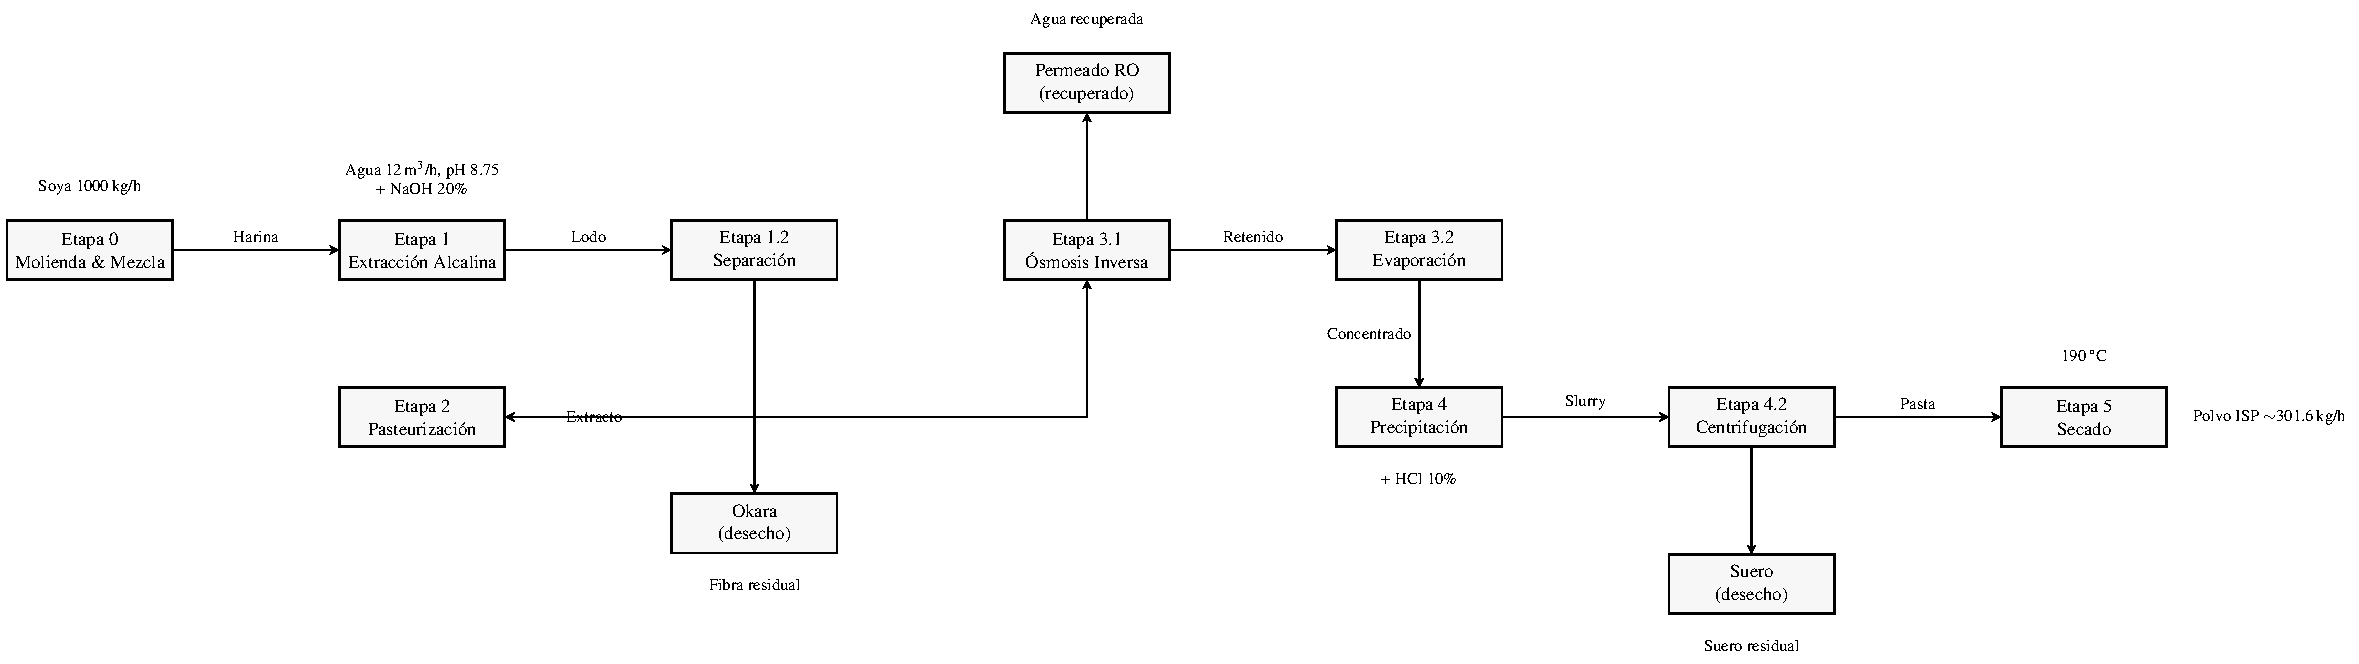
\includegraphics[width=0.85\textwidth]{figures/diagrama_flujo.pdf}
\caption{Process flow diagram of the ISP plant with the nine main stages.}
\label{fig:diagrama}
\end{figure}

\section{Architecture}

The system has four decoupled computational modules in the \texttt{core/} package, all in Python 3.10+. The modules communicate using structured dictionaries, which allows replacing one module without affecting the others.

\subsection{Module Overview}

\begin{itemize}
    \item \texttt{equipment\_}\allowbreak\texttt{specs.py} --- Equipment configuration. Defines \texttt{EQUIPMENT\_SPEC\_}\allowbreak\texttt{DEFAULTS} (nominal capacities), \texttt{EQUIPMENT\_SPEC\_}\allowbreak\texttt{LIMITS} (physical ranges), and \texttt{CAPACITY\_LIMIT\_}\allowbreak\texttt{DEFAULTS} (safety factors). Automatic validation via \texttt{validate\_equipment\_}\allowbreak\texttt{specs} and \texttt{validate\_capacity\_}\allowbreak\texttt{limits}.
    \item \texttt{stage\_equations.py} --- Phenomenological kernel. Independent \texttt{calc\_stage\_N} functions solve mass and energy balances for each stage. \texttt{run\_process\_}\allowbreak\texttt{model} orchestrates the sequence, validates numerical results, computes the global mass balance closure, and calls the constraint engine.
    \item \texttt{equipment\_constraints.py} --- Constraint engine. \texttt{evaluate\_capacity\_}\allowbreak\texttt{constraints} checks the load against equipment capacity adjusted by safety factors. \texttt{enforce\_capacity\_}\allowbreak\texttt{constraints} raises the error \texttt{Equipment}\allowbreak\texttt{CapacityError} when a limit is exceeded.
    \item \texttt{process\_model.py} --- History support. Provides \texttt{ControlLog} (circular buffer with 1,000 points) and \texttt{build\_snapshot} for organizing controls, specs, and results.
\end{itemize}

The control room interface (\texttt{app.py}) uses Streamlit to integrate a simulation loop with configurable step size, first-order process inertia, and real-time KPI visualization.

\subsection{Phenomenological Model}

Each stage solves algebraic mass and energy balances. The equations below show the ideal balances; the implementation incorporates penalty functions for off-nominal conditions, an operational loss factor ($F_{\text{LOSS}}=2\%$ per stage), and empirical efficiency maps.

The grinding and mixing stage combines soy and water:

\begin{equation}
\dot{m}_{0} = \dot{m}_{\text{soya}} + \rho_w Q_w \label{eq:stage0}
\end{equation}

with $\dot{m}_{\text{soya}} = 1{,}000\,\text{kg/h}$ and $\rho_w = 1{,}000\,\text{kg/m}^3$.

Alkaline extraction solubilizes protein. Extraction efficiency $\eta_{\text{ext}}$ is modulated by pH, temperature, residence time, and solid-liquid ratio penalties:

\begin{align}
\dot{m}_{\text{prot}} &= \eta_{\text{ext}} \, X_{\text{prot}} \, \dot{m}_{\text{soya}} \label{eq:stage1} \\
\eta_{\text{ext}} &= \eta_{\text{base}} \cdot f_{\text{pH}} \cdot f_T \cdot f_t \cdot f_r \label{eq:eff}
\end{align}

where $X_{\text{prot}} = 0.375$, $\eta_{\text{base}} = 0.88$, and each $f_i$ is a continuous penalty function that degrades efficiency outside the optimal window (pH~8.0--9.5, temperature~45--75$\,^\circ$C, residence~$\geq$60~min, ratio~9--14).

Reverse osmosis pre-concentration follows a simplified transmembrane pressure model:

\begin{equation}
\dot{m}_{\text{perm}} = \dot{m}_{\text{perm,ref}} \cdot \frac{\dot{m}_{\text{soya}}}{\dot{m}_{\text{soya,ref}}} \cdot \min\left(\frac{P}{P_{\text{ref}}}, 1.5\right) \label{eq:ro}
\end{equation}

Isoelectric precipitation at pH~4.5 and spray drying complete the sequence. The temporal response to setpoint changes uses a first-order filter:

\begin{equation}
y[k+1] = y[k] + (u[k] - y[k])(1 - e^{-\Delta t / \tau}) \label{eq:inertia}
\end{equation}

where $\tau$ is the time constant per variable, enabling heterogeneous dynamics across stages.

\subsection{Constraint Engine}

Capacity constraints compare process load against equipment capacity, adjusted by safety factors $f_s$:

\begin{align}
V_{\text{TK}} &\leq V_{\text{TK,max}} \cdot f_{s,\text{TK}} \label{eq:c1} \\
\dot{Q}_{\text{HX}} &\leq A_{\text{HX}} \cdot U \cdot \Delta T_{\text{lm}} \cdot f_{s,\text{HX}} \label{eq:c2} \\
\dot{m}_{\text{vap}} &\leq \dot{m}_{\text{vap,max}} \cdot f_{s,\text{EV}} \label{eq:c3}
\end{align}

When a violation occurs, the system raises \texttt{Equipment}\allowbreak\texttt{CapacityError} with a structured alarm that includes the equipment code, the load magnitude, and a recommendation for correction.

\section{Replicability Requirements}

Adapting the architecture to a new process requires three steps: (1) map the equipment and create \texttt{EQUIPMENT\_SPEC\_}\allowbreak\texttt{DEFAULTS} with design capacities, (2) implement the function \texttt{stage\_n}\allowbreak\texttt{(controls,}\allowbreak\texttt{ specs)} for each unit operation, and (3) define \texttt{CONTROL\_}\allowbreak\texttt{LIMITS} with the operational ranges. The validation functions make sure all parameters stay within physically possible values.

\section{Validation: ISP Plant Case Study}

The architecture was applied to an Isolated Soy Protein (ISP) plant at 1,000~kg/h nominal capacity \cite{lusas1995soy,kinsella1979}. The process has nine stages: grinding and mixing (E0), alkaline extraction (E1), primary separation (E1.2), HTST pasteurization (E2), reverse osmosis pre-concentration (RO), vacuum evaporation (E3), isoelectric precipitation (E4), centrifugation (E4.2), and spray drying (E5).

\subsection{Baseline Validation}

With nominal parameters ($\dot{m}_{\text{soya}} = 1{,}000\,\text{kg/h}$, $Q_{\text{water}} = 12\,\text{m}^3/\text{h}$, pH~8.75, $T_{\text{pasteur}} = 80\,^\circ$C, $\text{pH}_{\text{precip}} = 4.5$), the model produces:

\begin{itemize}
    \item Extraction efficiency: 88.0\%
    \item Protein precipitated: 292.3~kg/h
    \item Final powder: 301.6~kg/h (286.5~kg/h protein)
    \item Global protein yield: 76.4\%
    \item Mass balance closure error: $<$0.1\%
\end{itemize}

All eleven unit tests pass, confirming numerical integrity.

\subsection{Stochastic Diagnosis}

A Monte Carlo campaign of 10 batches $\times$ 10,000 runs (100,000 total) was carried out on the initial equipment design. All 19 control variables were randomly varied within wide ranges. Only 4.70\% of the runs were successful ($\sigma = 0.18\%$, 95\% CI: $[4.59\%, 4.81\%]$). The main bottlenecks were: extraction tank TK-101 (78.23\% of failures), water tank TK-100 (69.50\%), evaporator EV-301 (57.06\%), and heat exchanger HX-201 (40.69\%).

\subsection{Optimized Design}

Based on the diagnosis, the bottleneck equipment was resized (Table~\ref{tab:limits}). A second campaign of 30 batches $\times$ 10,000 runs (300,000 total) with wider operational ranges ($\pm20\%$ for feed rate, $\pm25\%$ for water flow) gave the following results:

\begin{itemize}
    \item \textbf{Success rate:} 99.88\% (299,633/300,000)
    \item \textbf{Std. deviation:} $\pm0.026\%$, 95\% CI: $[99.87\%, 99.89\%]$
    \item \textbf{Sigma level:} $Z = 3.03\sigma$ ($\sim$1,200 DPMO)
    \item \textbf{Residual failures:} Only \texttt{STAGE1\_TANK\_CAPACITY} in 0.12\%
\end{itemize}

\begin{table}[!ht]
\centering
\caption{Optimized capacity limits.}
\label{tab:limits}
\small
\begin{tabular}{lcc}
\toprule
Equipment & Variable & Limit \\
\midrule
TK-100 & Geometric capacity & 22.0 m$^3$ \\
TK-101 & Geometric capacity & 35.0 m$^3$ \\
HX-201 & Heat exchange area & 68.5 m$^2$ \\
EV-301 & Evaporative capacity & 16.0 m$^3$/h \\
CF-401 & Hydraulic flow & 10.0 m$^3$/h \\
SD-501 & Evaporative capacity & 1,000 kg/h \\
\bottomrule
\end{tabular}
\end{table}

\subsection{Energy Analysis}

Reverse osmosis removes 2,718.3~kg/h of water in liquid phase using only 8.5~kW of electrical power. This reduces the evaporator thermal load by 836.2~kW (19.5\%). The net savings of 827.7~kW allow the membrane investment to be recovered in less than 1.5 years.

\begin{table}[!ht]
\centering
\caption{Energy comparison: without RO vs with RO.}
\label{tab:energy_comparison}
\small
\begin{tabular}{lcc}
\toprule
Variable & Without RO & With RO \\
\midrule
Water removed by evaporation (kg/h) & 6,841.0 & 5,509.0 \\
Water removed by RO (kg/h) & 0.0 & 2,718.3 \\
Evaporator thermal power (kW) & 4,294.6 & 3,458.4 \\
Thermal savings (kW) & 0.0 & 836.2 (19.5\%) \\
RO electrical power (kW) & 0.0 & 8.5 \\
Net savings (kW) & 0.0 & 827.7 \\
\bottomrule
\end{tabular}
\end{table}

\begin{figure}[!ht]
\centering
\includegraphics[width=0.85\textwidth]{figures/monte_carlo_dist.pdf}
\caption{Distribution of success rates per batch for the optimized campaign (30 batches of 10,000 runs). The KDE curve approximates a Gaussian; the dashed red line marks the mean (99.88\%); dashed gray lines delimit the 95\% CI ($\pm0.026\%$).}
\label{fig:mc_dist}
\end{figure}

\section{Conclusion and Future Work}

We presented a modular, open-source Digital Model architecture validated through Monte Carlo simulation of an ISP plant. The key features that make it replicable are: externalized configuration with automatic validation, independent and replaceable stage equations, a decoupled constraint engine, and automated unit testing.

The stochastic diagnosis improved the design from 4.70\% to 99.88\% success (3.03$\sigma$), and the energy analysis showed a 19.5\% savings from RO integration. These results show that the architecture can be used for systematic process diagnosis and optimization during the conceptual design phase.

The source code is publicly available under MIT license, including the phenomenological kernel, constraint engine, and 11 unit tests. The Monte Carlo experiments can be reproduced with \texttt{python scripts/plot\_monte\_carlo.py}. Future work includes: IoT integration for Digital Shadow transition, multi-plant composition using the OpenTwins approach, and hybrid AI models for product quality prediction.

\section*{Acknowledgements}
\if1\blind
Acknowledgements are purposely removed for blind review.
\fi
\if0\blind
The author expresses sincere gratitude to Ing. Francisco Dilillo (instructor of the Unit Processes course) for his valuable guidance and support in this research.
\fi

\bibliographystyle{ieeetr}
\AtBeginEnvironment{thebibliography}{%
  \setlength{\itemsep}{0pt}%
  \setlength{\parskip}{0pt}%
  \setlength{\parsep}{0pt}%
}
\bibliography{references}

\end{document}
